\section{Data Enhancement}
\label{section: tracking method - data enhancement}


The data that comes from the mmWave sensor is quite sparse, thus, it's important to get as much information out of this data as we can, this process is called \textit{data enhancement}.
Data enhancement broadly covers any method that increases the "\textit{quality}" of the data that is being sent to the recognition systems.
This can be done in two major ways: firstly, the physical setup can be changed to increase the quality of the data, secondly, software systems can be put in place to add extra context to the raw data.
The first option, a change to the physical setup, can be quite effective, however, this should be avoided for the final product as it limits the flexibility of the system.
However, physical setup changes can help greatly during the design of a system, as you need good data to design a good interpretation system, and you need a good interpretation system to verify your data enhancement methods.
% One way in which this can be done is by changing the physical setup for the point gathering, though we would like to avoid this for the final product, as this could greatly limit the flexibility of the system.
Software-based data enhancement is more difficult to create, but also more flexible, which makes it a preferable option for the final system.
These systems work by adding additional information to the data already present, this is also where the difference between filtering and data enhancement exists.
Section \ref{section: tracking method - data filtering}, \textit{Data filtering}, also adds information, the label of "noise" vs "signal", but this is a subtractive (removing faulty data) process, as opposed to an additive (adding additional useful data) process, therefore, a distinction between filtering and enhancement is made.

\textbf{add a part about why we want to look at hands?}

\subsection{Physical Enhancement}
\label{sub-section: tracking method - data enhancement - physical enhancement}


Many similar HPE systems rely solely on physical wearables \cite{filippeshi2017survey, antonio2010the}. 
This is a logical choice, as it enables the direct tracking of specific parts of the user's body, at the cost of being more invasive and not easily deployable in non-private spaces.
In IAmMuse, a wearable was chosen that increases the reflectivity of a specific part of the user's body, namely their hands. Increasing the reflectivity
\begin{wrapfigure}{r}{0.32\textwidth}
    \caption{A reflective wearable}
    \centering
    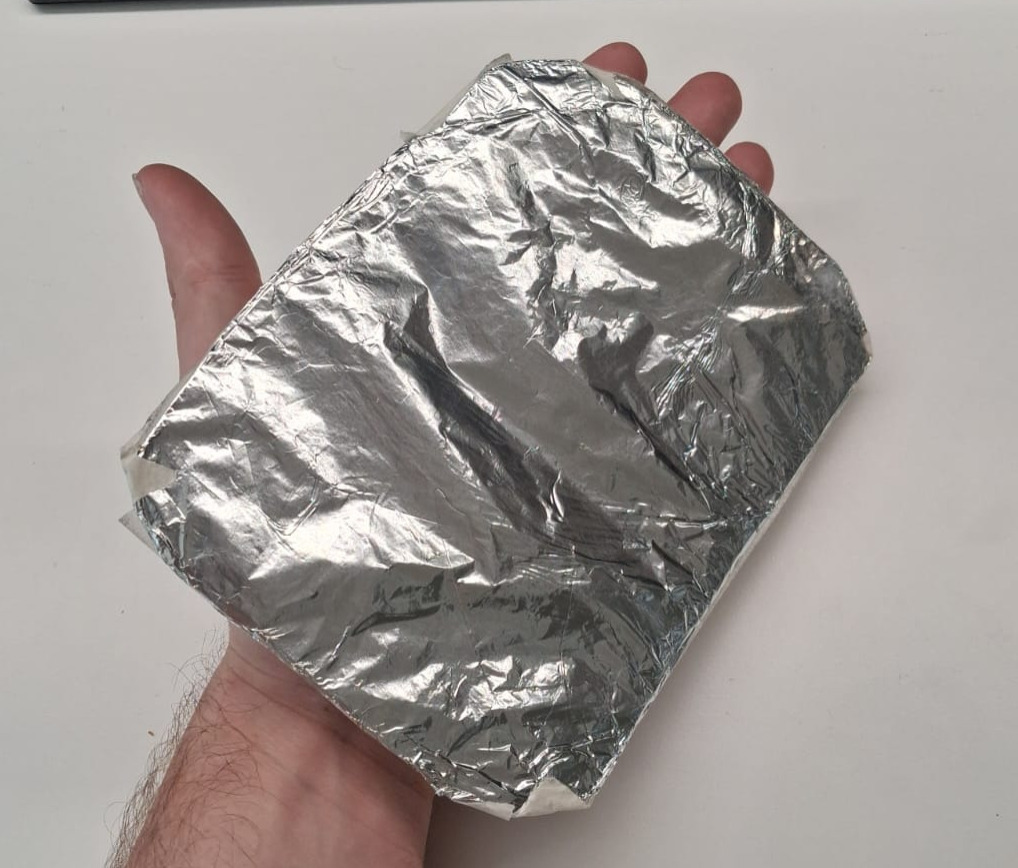
\includegraphics[width=0.32\textwidth]{figures/experimental setup/reflective wearable.png}
    \label{fig: reflective glove wearable}
\end{wrapfigure}
 at a certain location will make the mmWave radar generate more and denser point clusters at that location.
The reason IAmMuse wants a higher point density at the user's hands is due to the fact that the position of the hands is most indicative of the angle of a user's arm.
This is true because, for every angle change at the user's arm, the user's hand will move the largest distance, simply by being the part of the arm furthest removed from the shoulder.
For this reason, the hand is the most effective location to increase the reflectivity and thus point generation.
The software data enhancement method used by IAmMuse will, for the same reason, also increase the prevalence of the points belonging to the user's hands.




% One issue with data enhancement methods is that it's difficult to test enhancement methods if the system using the data does not work well yet, and it's difficult to test that a system is working well without good data enhancement methods.
% For this reason, it was decided that we would use a known \textit{physical} data enhancement method, in the form of a wearable (\cref{fig: reflective glove wearable}).
% This wearable could be worn on the hand and was covered in aluminum foil to increase the reflectivity of the hand.
% This caused the hands to produce more dense pointclouds, since the mmWave radar produces more points for more reflective surfaces.
% This, in turn, is useful since the hands are most indicative of the angle of someone's arm (assuming outstretched arms) as they are furthest away from the shoulder, and thus move the most when someone moves their arm.
% These reflective gloves ensured that the data used to create the later systems was of good quality while they were being designed.

% With the later parts of the pipeline in a decent state, it was possible to create software-based data enhancement methods and to "take off the gloves", so to speak.
% A significant part of this thesis was spent on creating and testing various systems of data enhancement, most of which did not produce adequate results, but which are still discussed in \cref{section: tracking method - different approaches}. 
% Furthermore, many of these systems rely, one way or another, on a "\textit{pre-configuration step}", where the user is asked to perform certain actions at startup for the system to initialize, which is discussed in \cref{section: tracking method - pre configuration}.
% Most of these data enhancement systems tried to "find" which points belonged to the hands, arms, and torso.
% This labeling would allow for weighing points of the hands more heavily, while weighing points of the arms less heavily and ignoring points of the torso, in effect, producing the same outcome as the gloves gave with their higher point density near the hands.

\subsection{Initialization, Minimal Enclosing Ball}
\label{sub-section: tracking method - data enhancement - minimal enclosing ball}

% Introduction software enhancement & MEB
As mentioned at the start of this section, the eventual goal is to create a software-based data enhancement system. 
IAmMuse's final enhancement system will be discussed here.
The eventual goal of this initialization would be to find out what points belong to what parts of the body.
If a distinction between points belonging to the torso, arms, and hands could be made, then IAmMuse can utilize this information in its interpretation system to more accurately predict the angles of the arms.
To achieve this, IAmMuse makes use of a \textit{Minimal Enclosing Ball} (MEB) over the user's data points, to get more information on the individual points. 
The goal of this system is to first create a point cloud that has points across the whole physical movement range of the user, in other words, it has points of the user's arms at all possible locations of their arms.
This point cloud is constructed during an \textit{initialization step}, where the user is asked to move their hands up and down until the initialization is complete.
IAmMuse then stacks these recorded frames until it has at least 3000 points, at which point IAmMuse informs the user that the initialization has been completed.
This point cloud should then contain noise points and points belonging to the user.
The user's points should roughly evaluate to a thin cylinder, where the center of the cylinder would be at the user's sternum, and the radius to the edge would be slightly larger than the user's arm span.
% The actual data in this point cloud (points belonging to the user, not to noise) should roughly evaluate to be a disk, with the user's sternum as a centroid and their arm span as a radius.
IAmMuse fits a ball around this data, and not a cylinder, because it's an easier and more explored problem, and it should be "good enough" in our case, given that the center and radius of such a ball should be very similar to the center and radius of an enclosing cylinder.
% In this method, we try to fit the smallest ball around the data, which encompasses all of the points belonging to the user while ignoring any noise points.

% MEB method
For this, we used a process described by \citeauthor{ding2020sublinear}, in \textit{algorithm 1} of their paper \cite{ding2020sublinear}.
This algorithm gives a stochastic estimation, with lower and upper bounds on the accuracy, of a minimal enclosing ball, with outliers.
Due to the stochastic nature of this method, it's possible to obtain a "bad result", which does not fit the underlying data correctly.
Even though this does not happen often, in order to mitigate the issue completely, IAmMuse calculates this estimation 100 times and uses the average of these results.
For the algorithm, we take $\delta$ (tightness bound) to be 0.08, we take $\gamma$ (noise percentage) to be 0.15, allowing 15\% of the points to be outside of the ball, and lastly we take $z$ (number of iterations used to look for an optimal solution) to be 50.
These exact numbers are a result of tuning the system to get the most consistent tight ball around the data points.
These variables should be re-examined if the system is deployed in a new environment, specifically $\gamma$ should be tuned to be as low as possible while avoiding taking noise points into account, and $z$ should be increased until the estimation does not improve any further.

% limitation, static ball.
A current limitation of this system is that a user can only \textit{initialize} the system once, and this initialization dictates where the user has to stand, since the system expects their sternum to be roughly at the center of the MEB.
A more dynamic version of the MEB initialization system was explored, where the MEB would be recalculated each frame with the most recent 3000 points.
This approach did not work well as the MEB started to drift at times, depending on the most recent positions the user held.
As an example, if a user wanted to hold their hands up high a lot, then after enough time, the point cloud used to generate the MEB would not be representative of the user's whole range of movement anymore.
Similar systems, which allow the user to move slightly during execution, are certainly feasible, but were deemed outside of the scope of this research and are thus left for future research.


\subsection{Programmatic enhancement: point weight}
\label{sub-section: tracking method - data enhancement - point weight}

% What we have (MEB); What we want ("hands" with higher weight)
Now that the system is initialized and has a ball that encompasses the full area of motion of the user's arms and is centered on the user's sternum, the actual data enhancement can be done.
Just as with the physical enhancement, discussed in \cref{sub-section: tracking method - data enhancement - physical enhancement}, we want to increase the "\textit{prevalence}" of the hands in the final point cloud.
The reflective gloves achieved this by increasing the reflectivity of the user's hands, and thus increasing the number of points produced at their location, by the mmWave sensor.
IAmMuse's enhancement system, on the other hand, tries to add an extra dimension of information to each point, namely a \textit{weight}.
This weight tells the interpretation system how well each point represents the potential position of the user's arm.

% Why we look at hands; How we "define"/find our hands
To determine how "representative" a specific point is, IAmMuse tries to determine how near to your hand that point is.
Here, the points that are likely to be generated by the user's hand will be given the highest weight, then the points that are most likely to have been generated by the user's arms will get a slightly lower weight, and the points belonging to the torso, or which are to far away from the user, should be given a low weight.
% The metric used to determine how "representative" a specific point is is to look at how near to your hand the point is.
% Since the absolute distance between two points, belonging to a frame where the user's arm was in a different zone (e.g. one frame with left low, and one frame with left mid), is the largest for the points produced by the hand, thus those are "most representative" of where the arm is currently located.
% The points belonging to the arm itself come after this, where the points at the wrist and lower arm are more representative than those at the elbow and upper arm.
As you might remember, the ball generated by our initialization closely encompasses the full area of motion of the user's arms, thus, we can estimate where the user's hands are, since the user's hands should always roughly trace the edge of this ball if they hold their arms outstretched.

% Restate question in terms of distance to MEB edge
This knowledge allows us to restate what the weight of a specific point is based on, from "how well does it represent the position of the arm" to "how close to the user's hand is this point", and finally, into "how close to the edge of the initialization ball is this point".
Where the previous ways to define weight were very difficult to calculate, as they relied on "real-world knowledge" of the user's position, this new definition does not require any such knowledge, as long as a proper initialization is performed.
The MEB estimation generated during initialization can be used as an estimate of the "real world situation", giving IAmMuse information on the user's position and arm span.
% using the estimation of the user's position and reach, as specified and calculated in \cref{sub-section: tracking method - data enhancement - minimal enclosing ball}.

% Gaussian kernel to calculate weight from distance
The distance between a point and the edge of the ball can be easily calculated as the distance between the center of the ball and the point in question, minus the radius of the ball.
The system should take into account the points at the edge itself, but should also take into account nearby points, just less so.
The system which was chosen to transform this distance into a specific weight was the \textit{Gaussian Function} because of its relative simplicity.
It can be used to devalue points which are further away from the edge, and allows that devaluing to be easily tuned by modifying one variable (the variance).
In practice, the distance between a point and the edge of the MEB is never directly calculated, rather, the Gaussian function is used for this.
Its expected value is equal to the radius of the circle, its variance is set to be 0.5m ($\sigma^2 = 0.25$), and the input value is the distance between the given point and the center of the MEB.
This gives each point a weight on the range $(0, 1]$, where points whose distance to the MEB center is closer to the radius of the MEB will get a higher score.
And higher scores mean that a point will be considered more strongly in the data interpretation.







% The data enhancement system, which ended up being used, was one where a \textit{Minimal Enclosing Ball with Outliers} (MEB) was used to get an idea of "where" the user was.
% For this, the user was asked to "wave around their arms", to collect pointclouds which covered the full range of arm movements of the user.
% The pointclouds from these frames were stacked until we had a pointcloud consisting of 3000 points, in which the majority of the points (all points excluding noise points) should be located in a disc around the user.
% The method described in \textit{algorithm 1} in \cite{ding2020sublineartimeframeworkgeometric} by Hu Ding was used to generate an approximate minimal-enclosing-ball from these points.
% This approximation is based on a random process, so in order to gain a more stable result, we averaged the results of 100 calculations.

% With this approximate knowledge of the users' \textit{position} (the center of the ball) and their \textit{arm span} (the radius of the ball), it becomes possible to assign a weight to the different points, based on how likely they are to belong to a hand.
% Conceptually, for any point, if its distance to the center of the MEB is similar to the radius of the MEB, then that point is very likely to have been emitted by a hand.
% If a point's distance the the center of the MEB is very different from the radius of the MEB, then the point will either be noise (if it's larger) or your arm/torso (if it's smaller).
% To apply this weight change, a Gaussian kernel was used, with $\sigma = 0.5$ and $x' = r$, r being the radius of the MEB.




% At points during the creation of the thesis, systems were used to enhance the quality of the data we received.
% The most important one of these was a reflective wearable you put on your hand, see \cref{fig: wearable}. 
% This wearable increased the density of points near the hand. This is particularly useful as the hand moves the most distance when you wave your arm.
% Due to this, it's easier to detect the arm position from hand points than from other arm points, as the effect of noise is reduced.

% One of the goals of this thesis, however, was to make a system that would work without the assistance of video cameras or wearables; thus, an alternative to this glove was made.
% One way to look at the effect of the wearable was that it moved the weighted average location of each arm towards the hand, as the hand produced more points.
% Another way to achieve this is by giving a higher weight to points further away from the body. 
% We could give every point a weight value of between 0.5 and 2, where the weight was linearly dependent on your distance from the center of the body. 
% The centrum of the body would then give you a weight of 0.5, any point 1 meter away from the body (or more) would gain a weight of 2, any points in between would get a weight proportional to their distance.

% This method emulates the desired result that the wearable provided without spawning any new points, as this could bring potential issues in and of itself. 
% The added information on each point (its weight) increases the quality of the data for our purposes, allowing us to get more accurate predictions on the locations of the arms.